\documentclass[12pt,a4paper]{tufte-handout}

\title{Sound}

\author[dishajk]{Disha Kuzhively}

%\date{28 March 2010} % without \date command, current date is supplied

%\geometry{showframe} % display margins for debugging page layout

\usepackage{graphicx} % allow embedded images
  \setkeys{Gin}{width=\linewidth,totalheight=\textheight,keepaspectratio}
  \graphicspath{{graphics/}} % set of paths to search for images
\usepackage{amsmath}  % extended mathematics
\usepackage{booktabs} % book-quality tables
\usepackage{units}    % non-stacked fractions and better unit spacing
\usepackage{multicol} % multiple column layout facilities
\usepackage{fancyvrb} % extended verbatim environments
  \fvset{fontsize=\normalsize}% default font size for fancy-verbatim environments
\usepackage{url}
\usepackage{hyperref}
\usepackage{tikz}
\usetikzlibrary{calc,patterns}
\usepackage[none]{hyphenat}
% Standardize command font styles and environments
\newcommand{\doccmd}[1]{\texttt{\textbackslash#1}}% command name -- adds backslash automatically
\newcommand{\docopt}[1]{\ensuremath{\langle}\textrm{\textit{#1}}\ensuremath{\rangle}}% optional command argument
\newcommand{\docarg}[1]{\textrm{\textit{#1}}}% (required) command argument
\newcommand{\docenv}[1]{\textsf{#1}}% environment name
\newcommand{\docpkg}[1]{\texttt{#1}}% package name
\newcommand{\doccls}[1]{\texttt{#1}}% document class name
\newcommand{\docclsopt}[1]{\texttt{#1}}% document class option name
\newenvironment{docspec}{\begin{quote}\noindent}{\end{quote}}% command specification environment

\newcommand{\hertz}{Hz}

\tikzset{
    pencil/.pic={
        \pgfmathsetmacro{\l}{3}
        \pgfmathsetmacro{\w}{\l/10}
        % Pencil body
        \fill[orange!80!yellow] (0,0) rectangle (\l,\w);
        % Wooden sharpened part
        \fill[brown!30] (\l,0) -- ({7*\l/6},\w/2) -- (\l,\w) -- cycle;
        
        \fill[black] ({7*\l/6},{\w/2}) -- ($({7*\l/6},{\w/2})!0.3!(\l,\w)$) --($({7*\l/6},{\w/2})!0.3!(\l,0)$) --cycle;
        % Edge lines

        \draw (0,0) rectangle (\l,\w);

        \draw (\l,0) -- ({7*\l/6},\w/2) -- (\l,\w);
        \fill[pink!60,draw=black] (-\w,0) rectangle (0,\w);
        \fill[gray!50, draw=black] (-\w/3,0) rectangle (0,\w);
    },
    speaker/.pic={
        \draw (-1,-1) --++ (1,0) --++ (2,-1)--++(0,3)--++(-2,-1)--++(-1,0);
        \node at (0,-.5) {Source of sound}; 
    }
}

\begin{document}

\maketitle% this prints the handout title, author, and date

\begin{abstract}
\noindent
This article was prepared by the author to serve as a draft for TNSCERT class 8 chapter on the concept of Sound for TNSCERT during the the Tamil Nadu Curriculum Framing(TNCF) workshop that was held in Asha Nivas, Chennai  from 13-11-2025 to 15-11-2025, and 09-03-2026 to 10-03-2026.

The right side margin of each page contains notes for teachers, and prompts to activities that the teacher can initiate in the classroom.
\end{abstract}

% \printclassoptions

Every day we experience many natural and human-made sounds around us: the school bell ringing, raindrops falling on the ground, a dog barking, or a phone ringing. \marginnote{Write down all the sounds that are familiar to you.} But how are these sounds produced? How do they propagate\footnote{Here the word 'propagate' is used instead of simpler and familiar word like 'travel' to avoid misconceptions that students create, e.g. The word travel suggests that 'sound' is a moving object. Words are chosen to ensure that students develop a scientifically accurate mental model of the concept.} from one place to another? Why do different sounds have different characteristics? In this chapter, we will explore how sound is produced and how it propagates. We will also learn to think of sound as a form of energy and understand it as a wave.

\section{How is Sound Produced?}\label{sec:production}
\subsection{Activity: Vibrating Scale}\label{sec:production-activity}

Materials required:
\begin{enumerate}
    \item Geometry box including scale
    \item Rubber bands
    \item Rough paper
    \item Scissors
\end{enumerate}

Hang the scale over the edge of the desk so that part of it sticks out. Push the free end of the scale downwards and then let it go.
\begin{marginfigure}
  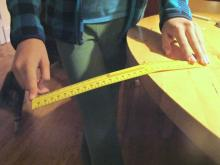
\includegraphics{scale-down}
  \caption[Sound with a scale]{Step 1. Push the free end of the scale downwards.}
\end{marginfigure}
\marginnote{\footnotesize Image credit: Ingrid Sulston, licensed under CC BY-NC-SA 4.0}
\begin{marginfigure}
  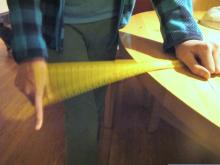
\includegraphics{scale-vibrate}
  \caption[Sound with a scale]{Step 2. Let the pushed end go.}
\end{marginfigure}
\marginnote{\footnotesize Image credit: Ingrid Sulston, licensed under CC BY-NC-SA 4.0}
\newthought{Observe:} Do you hear a sound? Do you see the scale move up and down rapidly? What kind of motion is the scale showing?

\subsection{Musical Geometry Box}
Empty your geometry box. Stretch a rubber band tightly around the box. Pluck or poke the rubber band.
\newthought{Observe:} Do you hear a sound? What part of the setup is moving?

\subsection{Paper whistle}
\begin{figure}[h]
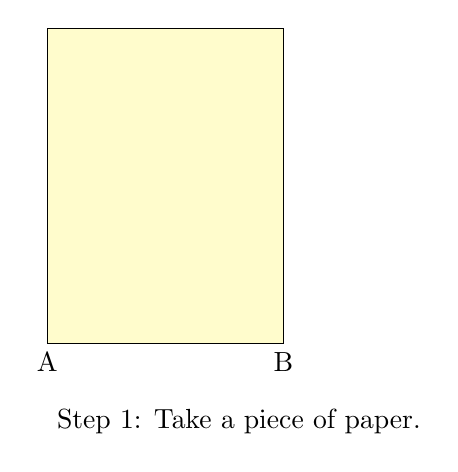
\begin{tikzpicture}
        \draw[fill=yellow!20] (0,0) node[below] {A} rectangle (3,4);
        \node[below] at (3,0) {B}; 
        \node[right] at (0,-1) {Step 1: Take a piece of paper.}; 
    \end{tikzpicture}
    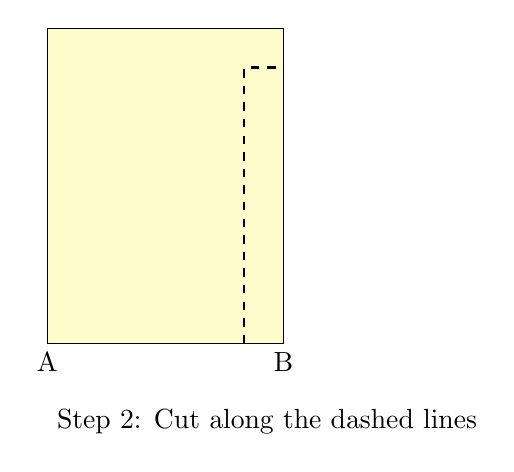
\begin{tikzpicture}
        \draw[fill=yellow!20] (0,0) node[below] {A} rectangle (3,4);
        \node[below] at (3,0) {B}; 
        \draw[dashed,thick] (2.5,0)--++(0,3.5) --++(0.5,0);
        \node[right] at (0,-1) {Step 2: Cut along the dashed lines}; 
    \end{tikzpicture}
    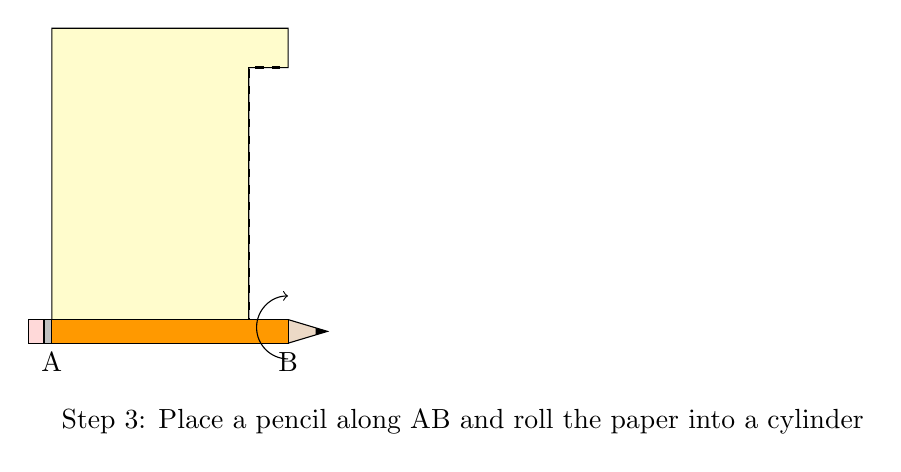
\begin{tikzpicture}
        \draw[fill=yellow!20] (0,0) node[below] {A} --++(2.5,0) --++ (0,3.5) --++(0.5,0) -- (3,4) --++ (-3,0) --cycle;
        \node[below] at (3,0) {B}; 
        \draw[dashed,thick] (2.5,0)--++(0,3.5) --++(0.5,0);
        \node[right] at (0,-1) {Step 3: Place a pencil along AB and roll the paper into a cylinder}; 
        \pic at (0,0) {pencil};
        \draw[->] (3,-.2) arc [start angle=270, end angle=90, radius=4mm];
    \end{tikzpicture}
    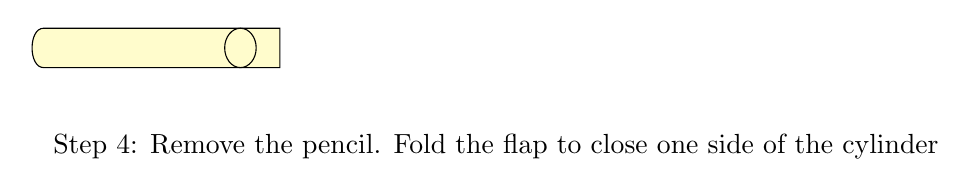
\begin{tikzpicture}
        % \draw[fill=yellow!20] (0,0) node[below] {A} --++(2.5,0) --++ (0,3.5) --++(0.5,0) -- (3,4) --++ (-3,0) --cycle;
        \node[right] at (0,-1) {Step 4: Remove the pencil. Fold the flap to close one side of the cylinder}; 
        \draw[fill=yellow!20] (0,0) to [out=180,in=180] (0,0.5) -- (3,0.5) -- (3,0) -- cycle;
        \draw (2.5,0.25) circle [x radius=0.2,y radius=0.25];
    \end{tikzpicture}
%  \checkparity This is an \pageparity\ page.%
  \caption{Instructions for creating your own sound maker.}
  \label{fig:ppfig1}
%   \zsavepos{pos:ppfig1}
  \setfloatalignment{b}
\end{figure}

Create your own paper whistle as shown in figure~\ref{fig:ppfig1}. Suck air in through the open end.

\subsection{Optional Activity: Tuning Fork}
\textit{This activity can be done if a tuning fork is available.}

Strike a prong of a tuning fork gently with a rubber hammer to make it vibrate. Bring the vibrating tuning fork close to your ear. Can you hear a sound? 

Gently touch the prongs of the vibrating tuning fork with your finger. What do you feel? Strike the tuning fork again. Lightly touch the vibrating prongs to the surface of water in a bowl. Do you see ripples forming on the surface of the water?
\begin{marginfigure}
  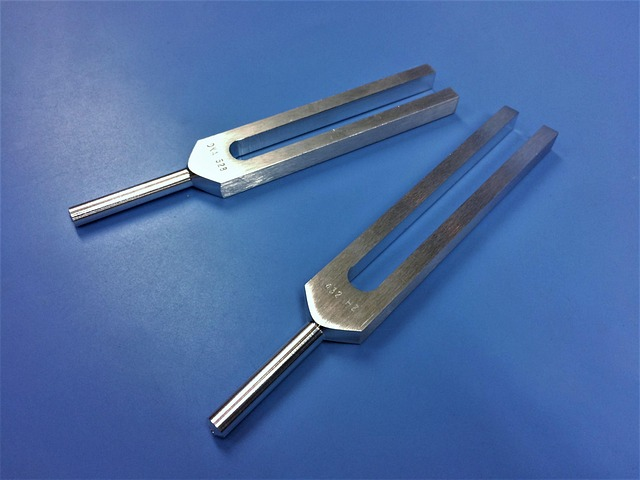
\includegraphics{tuning-fork}
  \caption[Tuning fork]{Tuning fork}
\end{marginfigure}

\newthought{Discussion:} In each case, some part of the object moves back and forth rapidly. This type of motion is called \textbf{vibration}. 

\newthought{Sound is produced when objects vibrate.}

The vibrating part of an object can cause nearby objects, such as air or water, to vibrate and form ripples. The vibrations propagate to us as sound.

Create a table as shown in Table~\ref{tab:obs-table} listing the object that produces sound and the part of the object that vibrates.

\begin{table}[ht]
  \centering
  \fontfamily{ppl}\selectfont
  \begin{tabular}{lll}
    \toprule
    Sl. No. & Object that produces sound & Part of the object that vibrates \\
    \midrule
    1 &Vibrating scale & Tip of the scale \\
    2 & Musical geometry box& \vdots \\
    3 &\vdots & \vdots \\
    \vdots &\vdots & \vdots \\
    \bottomrule
  \end{tabular}
  \caption{Observation table}
  \label{tab:obs-table}
  %\zsavepos{pos:normaltab}
\end{table}
\marginnote{Did you know? Many quartz clocks and watches keep time using a small quartz crystal. This crystal is shaped like a tiny tuning fork.}
\section{How Sound Propagates?}
\subsection{Activity}
Materials required:
\begin{enumerate}
    \item Mobile phone
    \item Airtight container
\end{enumerate}
Switch on music on the mobile phone and place it inside the airtight container. Close the lid of the container tightly.

\newthought{Observe:} What happens to the sound from the mobile phone?

\newthought{Discussion:} Sound propagates through air and reaches our ears. Sound cannot propagate through vacuum.

\subsection{Listening through wood or metal}

Place your ear on the desk. Ask your benchmate to gently tap the desk with a pencil a short distance away from your ear. Now compare listening with your ear in the air and listening with your ear touching the table.

\newthought{Observe:} The sound is usually louder or clearer through the table.

\newthought{Discussion:} Sound can propagate through solids, not just through air.

Sound needs a medium (such as air, water, or solids) to propagate. A material through which sound propagates is called a \textbf{medium}.

\subsection{Does air travel with the sound?}

Materials required:
\begin{enumerate}
    \item A piece of tissue paper or a candle
    \item A sound-producing object (such as a bell, or a plate and spoons)
\end{enumerate}

Place the candle (or hang the tissue paper) about 20-30 cm away from the sound source. Produce a sound.

\newthought{Observe:} Watch the flame or tissue carefully. It usually does not move much, or moves only slightly. If air were travelling from the sound source to your ear like wind, what should happen to the flame or tissue?

\newthought{Discussion:} In sound, the air particles vibrate back and forth in place. Each particle pushes the next one, passing the vibration along. The vibration propagates through the medium, not the particles themselves moving across the room In this activity, the air itself is not moving across the room.

\subsection{Sound Waves}
We have seen that sound is produced when objects vibrate. These vibrations make the surrounding air vibrate. Each air particle pushes the next one, passing the vibration along, like a chain of pushes. In this way, the vibration propagates through the air from the sound source to our ears. When vibrations move through a medium like this, they form a wave. Sound propagates through air as a sound wave.

\subsection{Compressions and Rarefactions}

When sound propagates through air, the air particles move back and forth around their positions. As they move, they sometimes come closer together and sometimes move farther apart. The regions where air particles are closely packed together are called \textbf{compressions}. The regions where air particles are farther apart are called \textbf{rarefactions}.

As a sound wave propagates through air, compressions and rarefactions move forward through the air. This pattern of compressions and rarefactions carries the sound from the source to our ears.

\begin{figure}[h]
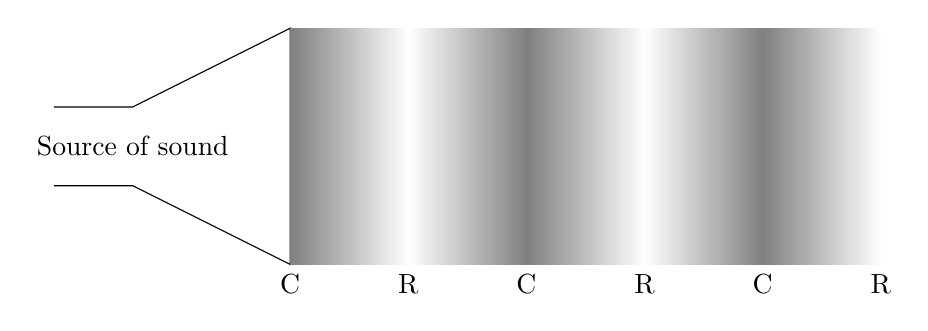
\begin{tikzpicture}
        \pic at (0,0) {speaker};
        \shadedraw[shading=axis,shading angle=90,draw=none] (2,-2) rectangle (3.5,1);
        \shadedraw[shading=axis,shading angle=-90,draw=none] (3.5,-2) rectangle (5,1);
        \shadedraw[shading=axis,shading angle=90,draw=none] (5,-2) rectangle (6.5,1);
        \shadedraw[shading=axis,shading angle=-90,draw=none] (6.5,-2) rectangle (8,1);
        \shadedraw[shading=axis,shading angle=90,draw=none] (8,-2) rectangle (9.5,1);
        \node[below] at (2,-2) {C};
        \node[below] at (3.5,-2) {R};
        \node[below] at (5,-2) {C};
        \node[below] at (6.5,-2) {R};
        \node[below] at (8,-2) {C};
        \node[below] at (9.5,-2) {R};
    \end{tikzpicture}
%  \checkparity This is an \pageparity\ page.%
  \caption{Sound propagates as density variations in the medium. C: Compression, R: Rarefaction}
  \label{fig:ppfig2}
%   \zsavepos{pos:ppfig1}
  \setfloatalignment{b}
\end{figure}

\subsection{Optional Activity: Slinky}

Take a slinky or a long spring. Ask your classmate to hold one end while you hold the other end. Stretch the slinky gently between you. Now give the slinky a quick push toward your classmate.
\begin{marginfigure}
  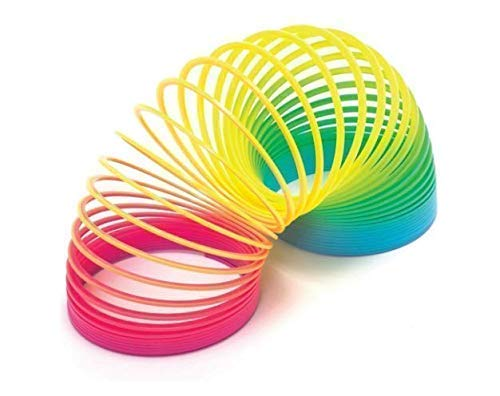
\includegraphics{slinky}
  \caption{Long spring also known as slinky.}
\end{marginfigure}
\newthought{Observe:} What happens when you push and pull the slinky back and forth along its length? Tie a ribbon somewhere in the middle of the slinky. Watch the ribbon carefully. You will notice that the ribbon moves back and forth, parallel to the direction in which the disturbance propagates.

This is how sound waves propagate: molecules bump the next molecules along, forming a wave of vibrations. These are called \textbf{longitudinal waves}, and is how sound propagates through solids, liquids and gases. 

\section{How Fast Does Sound Propagate?}
Do we hear sound instantly after it is produced? Think about what happens during lightning and thunder. When lightning strikes, we see a flash of light and hear thunder.

\newthought{Observe:} Do you see the lightning and hear the thunder at the same time? Or do they happen one after the other? Which do you notice first?

Usually, we see the lightning first and hear the thunder later.
\begin{marginfigure}
  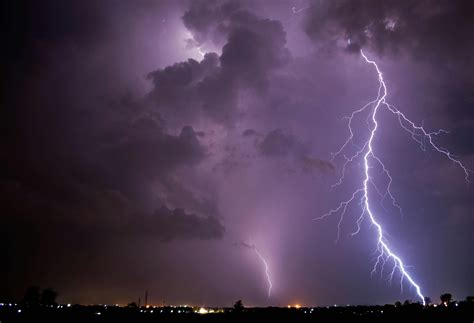
\includegraphics{thunder}
  \caption[Thunder and lightening]{Thunderstorm in Tiruchirappalli, Photo by Amol Mande}
\end{marginfigure}
Now think about what happens when crackers burst.

These observations show that sound takes time to propagate from the source to our ears. Light travels much faster than sound, so we see the flash before we hear the sound. 

In air, sound propagates at a speed of about 340 metres per second (at room temperature). Does sound propagate at the same speed through all mediums? 

Sound does not propagate at the same speed in all materials. The speed of sound depends on the medium through which it propagates. Sound propagates fastest in solids, slower in liquids, and slowest in gases. For example, sound propagates faster in metal or wood than in air. This is because the particles in solids are closer together, allowing vibrations to pass more quickly from one particle to the next. 

How does temperature affect the speed of sound?

\marginnote{As the temperature increases, the speed of sound increases. This happens because when the temperature is higher, the particles of the medium move faster. As a result, they pass the vibrations to neighbouring particles more quickly, allowing sound to propagate faster. For example, sound travels faster in warm air than in cold air.}

\subsection{Activity: Vibrating Scale}
Place a scale on the edge of a desk so that part of it hangs over the edge. Hold the scale firmly on the desk and pluck the free end so that it vibrates and produces a sound. Optionally, you may use a phone to record a video of the scale in slow-motion setting.

\newthought{Observe:} How does the sound and speed of vibration change as you change the length of the overhanging edge? How fast does the scale vibrate? 

You may notice that when the scale is longer, it vibrates more slowly and the sound is lower and when the scale is shorter, it vibrates faster and the sound is higher. If you have a slow motion recording, you can replay the video and count how many times the scale moves back and forth in 5 second and divide the number by 5 to find out how many times it moved back and forth in one second.

When the scale vibrates, it also makes the surrounding air vibrate. As the scale moves back and forth, it pushes and pulls the nearby air. This creates regions where the air is slightly compressed and regions where it is spread out. These compressions and rarefactions propagate through the air as sound waves. When the sound waves reach our ears, they cause the eardrum to vibrate, which allows us to hear the sound.

\newthought{Discussion:} the number of vibrations that occur in one second is called the \textbf{frequency} of the vibration. Frequency is measured in hertz (\hertz) and usually represented by the Greek letter $\nu$ (nu). Frequency tells us how often an event occurs in a unit of time. 

\newthought{Example:} if you beat a drum 10 times in one second, the frequency of your beating is 10 \hertz.

Sounds with higher frequency have a higher pitch and sounds with lower frequency have a lower pitch. A mosquito makes a high-pitched sound. A drum makes a low-pitched sound. Which one is vibrating faster?

When the scale vibrates, it sets the surrounding air into vibration. As the scale moves back and forth, it creates regions where the air is slightly compressed and regions where the air is slightly spread out. These compressions and rarefactions move through the air as sound waves. When they reach our ears, they cause the eardrum to vibrate, allowing us to hear the sound.

\marginnote{Kavin and Trisha are standing at different distances from the lightning. Both hear the thunder. Will the pitch of the thunder be different for Kavin and Trisha? Will the loudness of the thunder be different?}

You may also have noticed something else during the activity. When the scale was plucked gently, the sound was soft. When the scale was plucked harder, the sound was louder. If you watch the scale carefully, you will see that when it is plucked harder, it moves farther away from its resting position during each vibration. 

The size of this vibration is called the \textbf{amplitude}. Amplitude tells us how large the vibration is. A vibration with greater amplitude produces a louder sound, while a vibration with smaller amplitude produces a softer sound. Amplitude affects loudness, not pitch.

\marginnote{Two sounds have the same pitch, but one is louder. What must be different?}
\subsection{Hearing loss and hearing aids}
Very loud sounds can damage the inner ear and lead to hearing loss. Some people are born with conditions that affect their ability to hear. 
\begin{marginfigure}
  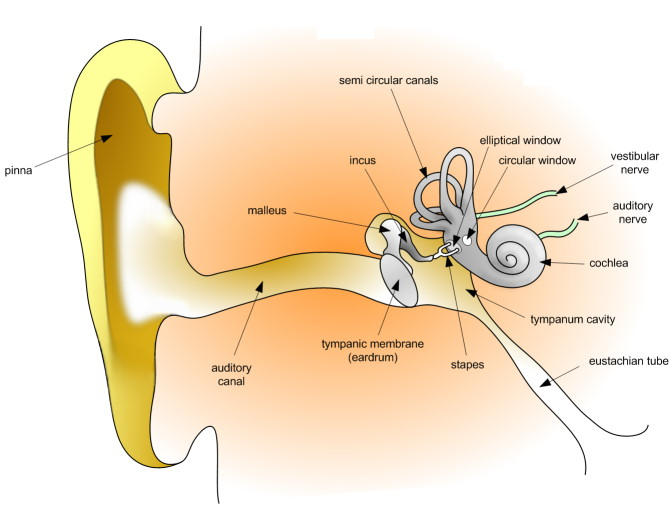
\includegraphics{HumanEar}
  \caption{Diagram of the auditory system of the human ear. Illustration by Dan Pickard.}
\end{marginfigure}
Hearing aids are devices that help such people hear better. They work by amplifying sound, that is, by increasing the amplitude of the sound waves.
\begin{marginfigure}
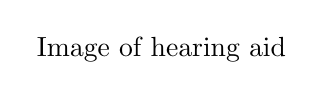
\begin{tikzpicture}
  \node at (0,0) {Image of hearing aid};
\end{tikzpicture}
  \caption{Image of hearing aid}
\end{marginfigure}

\marginnote{Pitch depends on frequency, which is determined by the source. Distance from the source does not change the frequency. As sound spreads out, its amplitude decreases, this is why it becomes quieter as you move far from the source.}

\subsection{Musical instruments}
Musical instruments produce sound by making strings, membranes, or air columns vibrate. By changing certain parts of the instrument, musicians can change the frequency of vibration, and therefore the pitch of the sound.

Different instruments change the frequency in different ways.

Veena (string instrument): The strings vibrate to produce sound. Pressing the string at different positions changes the length of the vibrating string, which changes the frequency and the pitch.
\begin{marginfigure}
  
\includegraphics{veena}
  \caption{Veena from Chennai, Wikimedia Commons}
\end{marginfigure}

Parai (drum): The stretched membrane (skin) vibrates when it is struck. Changing the tightness of the membrane changes the frequency of vibration and the sound produced.
\begin{marginfigure}
  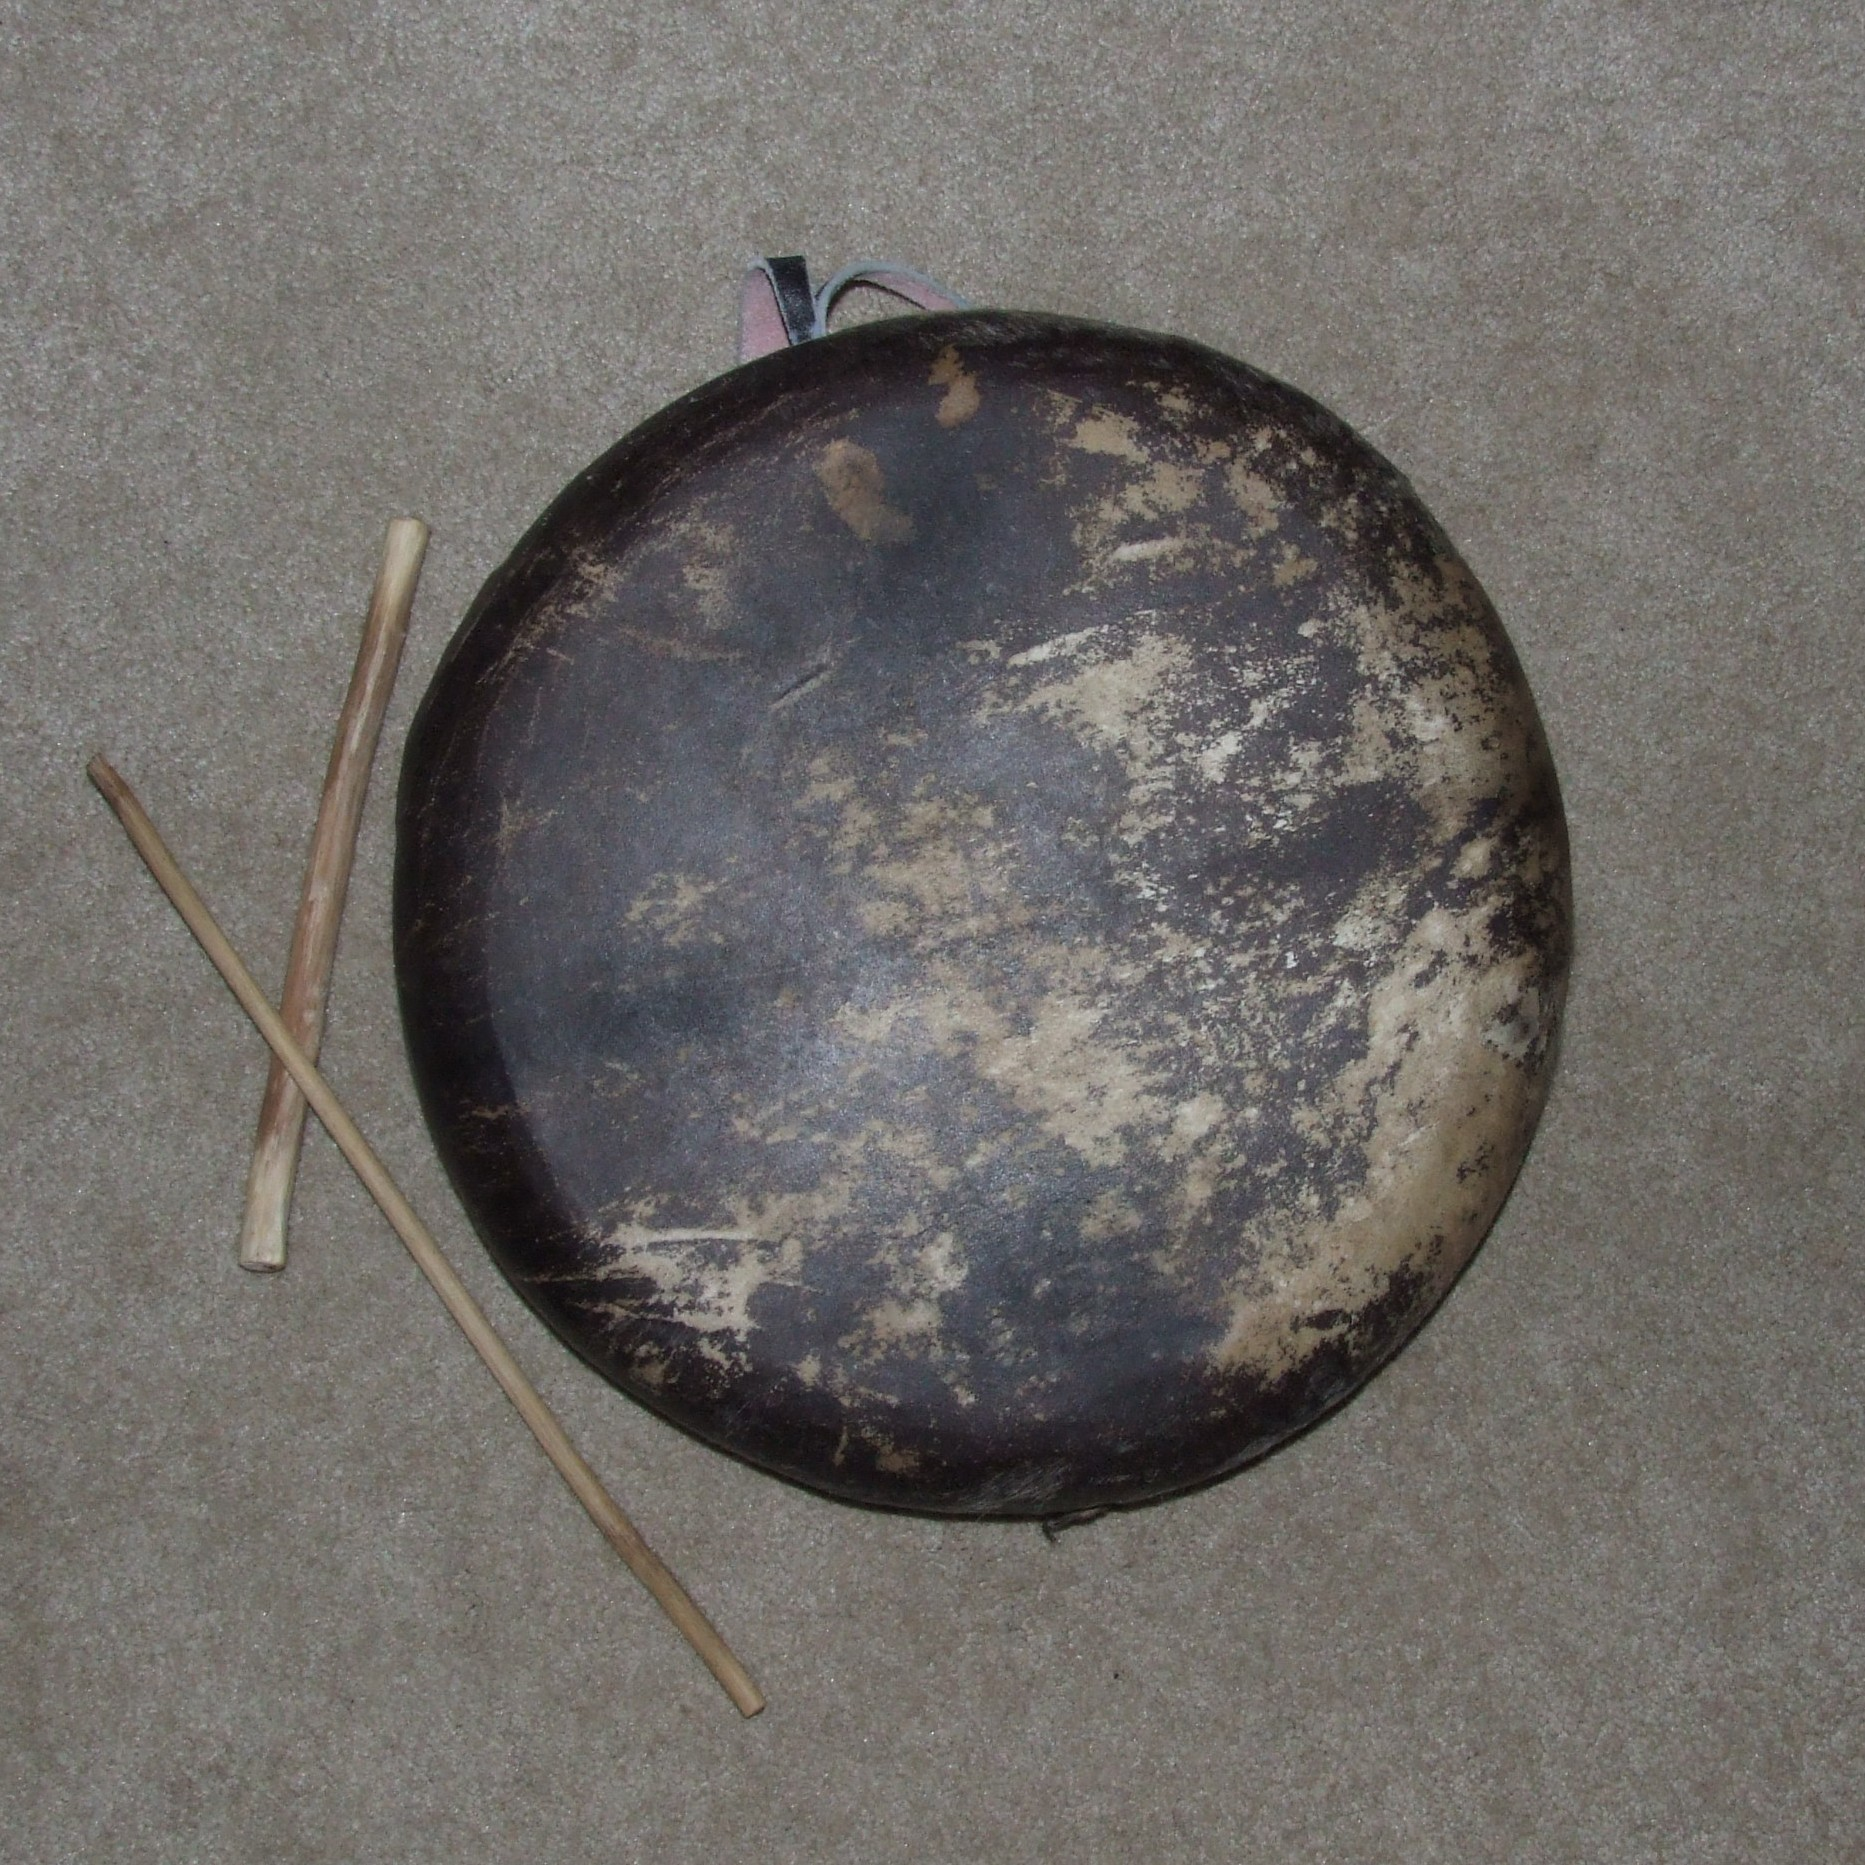
\includegraphics{parai}
\caption{Front side of a parai with the sticks used to play the instrument. Image by Prabhunkl, licensed under CC BY-SA 4.0}  
\end{marginfigure}
Nadaswaram (wind instrument): Sound is produced by vibrations of the air column inside the instrument. Opening and closing the finger holes changes the effective length of the air column, which changes the frequency.
\begin{marginfigure}
  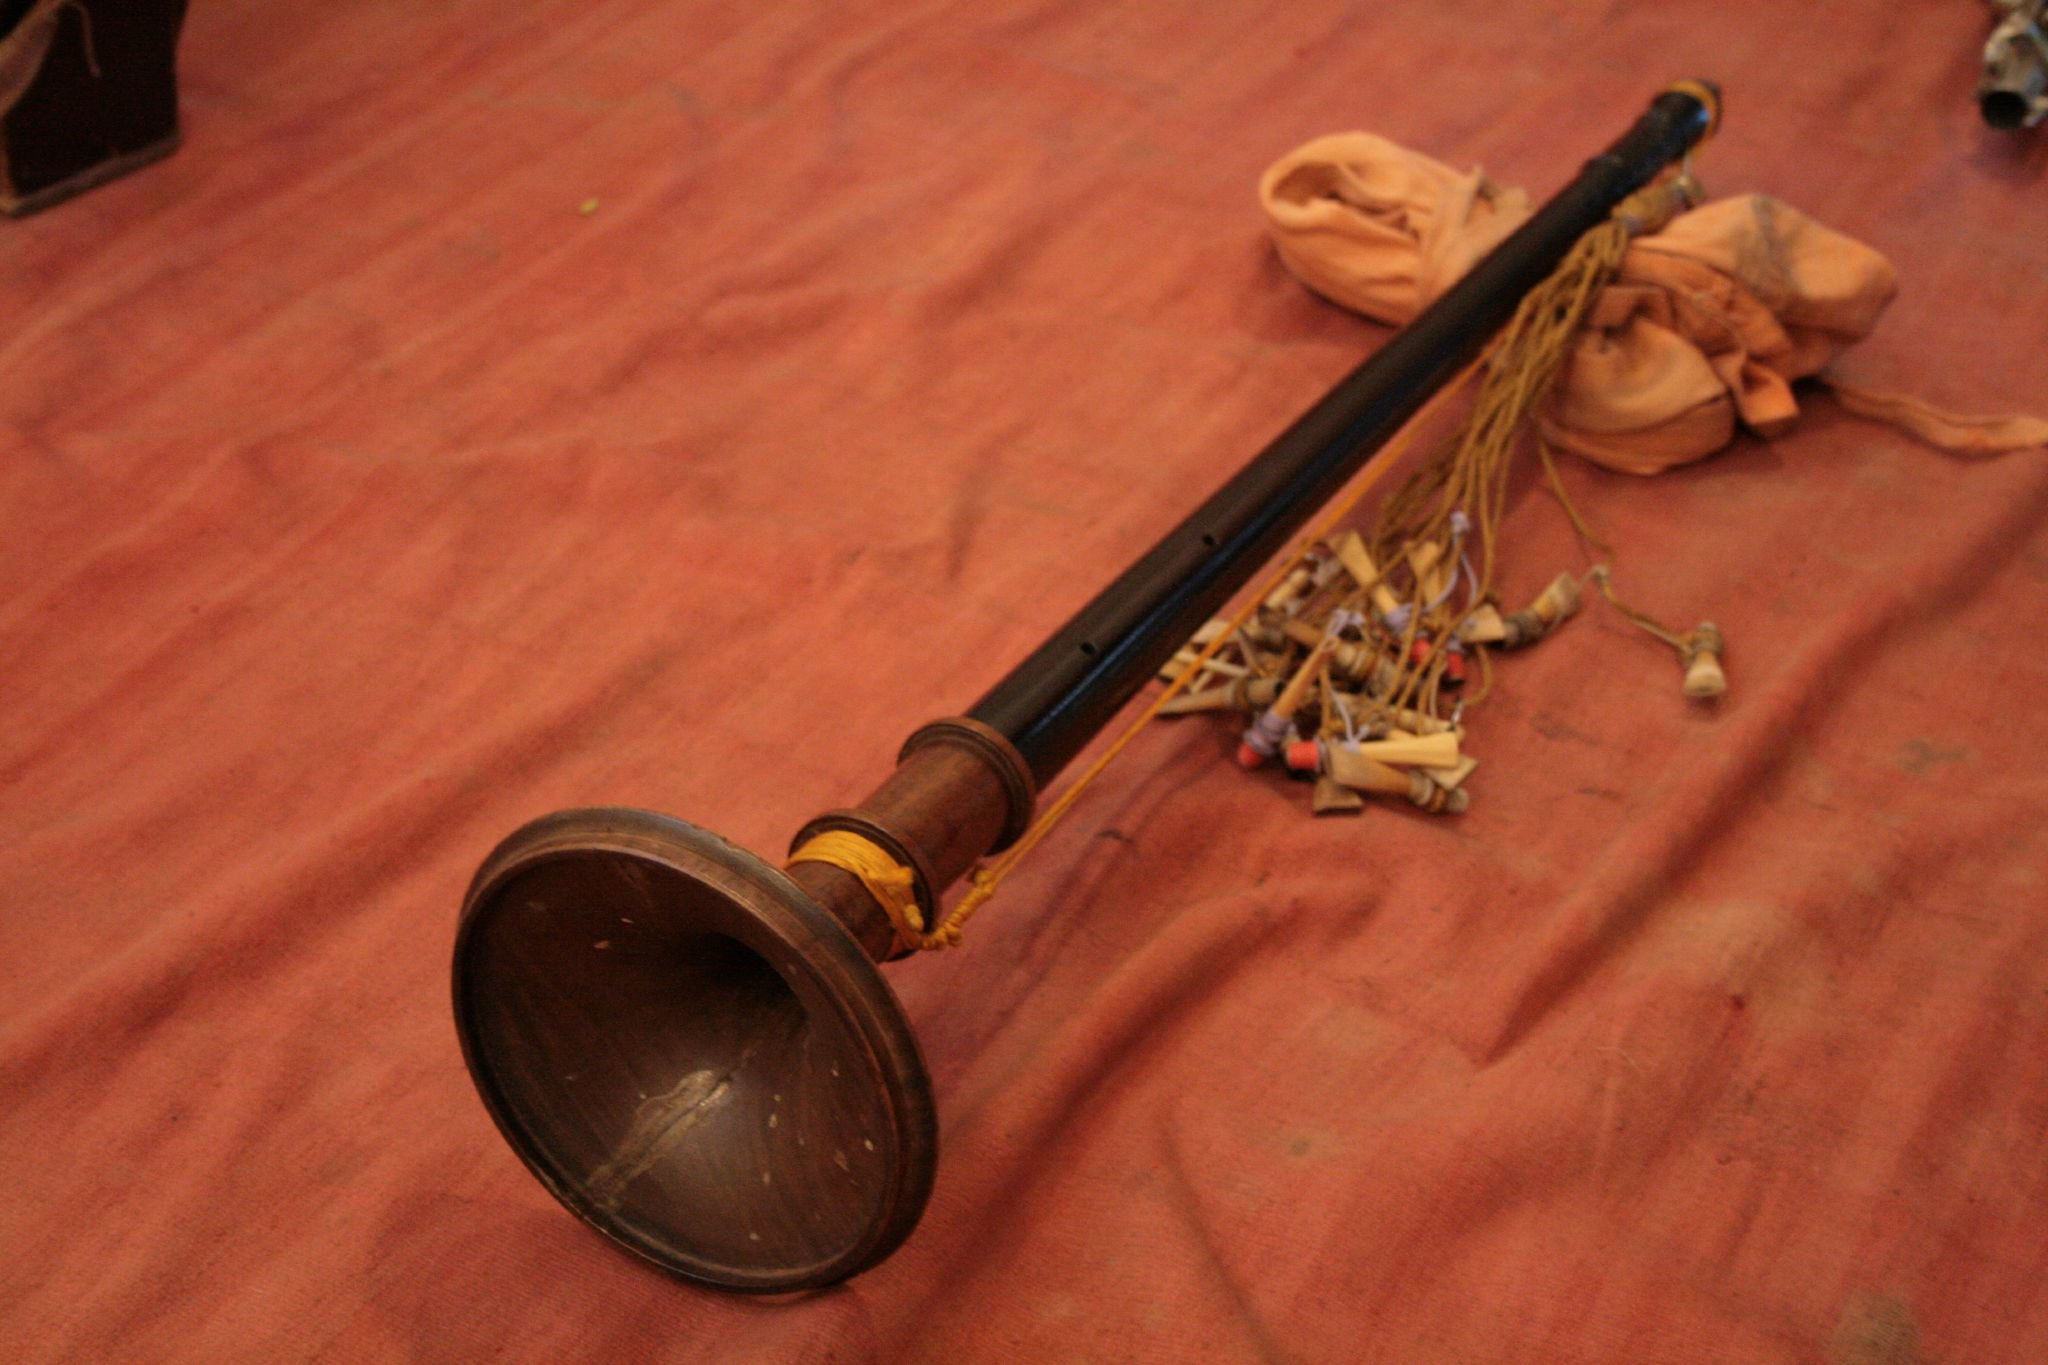
\includegraphics{nadaswaram}
\caption{Nadaswaram (also nagaswaram or nagasuram), Image by Ashwin Kamath}
\end{marginfigure}
Although these instruments look very different, they all produce sound through vibrations, and the frequency of vibration determines the pitch of the sound.

\subsection{Ultrasound}
Humans can hear sounds with frequencies roughly between 20 \hertz and 20,000 \hertz. Sounds with frequencies higher than 20,000 \hertz are called ultrasound. Humans cannot hear ultrasound.

Ultrasound has many useful applications:

\begin{enumerate}
\item Medical imaging: Doctors use ultrasound to look inside the body, for example to observe a developing fetus during pregnancy.
% \begin{marginfigure}
%   \includegraphics{ultrasound}
% \caption{Image of Ultrasound Machine}
% \end{marginfigure}
\item Detecting cracks in materials: Ultrasound can be used to find cracks or defects in metals and other materials.
\item Animal communication and navigation: Some animals, such as bats and dolphins, produce and detect ultrasound. They use it to communicate and to find objects around them.
\item Ultrasound is also used in a process called echolocation, where animals detect objects by listening to the echoes of the sound waves they produce.
\begin{marginfigure}

\includegraphics{bat}
\caption{Greater Indian fruit bat, image by Praveenp, licensed under CC BY-SA 4.0}
\end{marginfigure}
\end{enumerate}

\subsection{Activity: Slinky}

Take a slinky or a long spring. Ask your classmate to hold one end while you hold the other end. Stretch the slinky gently between you. Now give the slinky a quick push toward your classmate.

\newthought{Observe:} a compression moves along the slinky. You will see regions where the coils are close together and regions where the coils are spread apart. The region where the coils are close together is called a compression. The region where the coils are farther apart is called a rarefaction. This is similar to what happens in sound waves in air.

The distance between two neighbouring compressions (or two neighbouring rarefactions) is called the \textbf{wavelength}. Wavelength is measured in the units of distance. Remember, metre is the SI unit of distance.

Repeat the activity, but now create compressions more quickly.

\newthought{Observe:} The compressions become closer together, so the wavelength becomes shorter. If vibrations happen more often each second (higher frequency), the compressions are packed closer together and the wavelength becomes shorter.

When sound travels through a medium, regions of compression and rarefaction move through the medium. The distance between compressions is the wavelength. The speed of a sound wave depends on both its frequency and its wavelength.


\begin{equation}
\text{Speed} = \text{Frequency}\times\text{Wavelength}
\end{equation}

\marginnote{If the thunder sounds quieter when you are farther away, does the thunder have less energy when it reaches you?}

\subsection{Echo}
sound travels at a finite speed
sound can reflect from surfaces
An echo is heard when reflected sound reaches our ears after a short delay.

\subsection{Noise Pollution}
traffic noise
loudspeakers
industrial noise
How can we reduce noise pollution in cities?



Sound is one example of a mechanical wave that is longitudinal. There is also another type of wave, called
a transverse wave. In a transverse wave
particles do not oscillate along the direction
of wave propagation but oscillate up and down
about their mean position as the wave travels.
Thus, a transverse wave is the one in which
the individual particles of the medium move
about their mean positions in a direction
perpendicular to the direction of wave
propagation.
When we drop a pebble in a
pond, the waves you see on the water surface
is an example of transverse wave. Light is a
transverse wave but for light, the oscillations
are not of the medium particles or their
pressure or density — it is not a mechanical
wave. 


\nocite{PhysRevSTPER.6.020114}

\bibliographystyle{plainnat}
\bibliography{sound}

\end{document}
This style provides \textsc{a}- and \textsc{b}-heads (that is,
\Verb|\section| and \Verb|\subsection|), demonstrated above.

The Tufte-\LaTeX\ classes will emit an error if you try to use
\linebreak\Verb|\subsubsection| and smaller headings.

% let's start a new thought -- a new section
\newthought{In his later books},\cite{Tufte2006} Tufte
starts each section with a bit of vertical space, a non-indented paragraph,
and sets the first few words of the sentence in \textsc{small caps}.  To
accomplish this using this style, use the \Verb|\newthought| command:  
\begin{docspec}
  \doccmd{newthought\{In his later books\}, Tufte starts\ldots}
\end{docspec}

\subsection{Sidenotes}\label{sec:sidenotes}
One of the most prominent and distinctive features of this style is the
extensive use of sidenotes.  There is a wide margin to provide ample room
for sidenotes and small figures.  Any \Verb|\footnote|s will automatically
be converted to sidenotes.\footnote{This is a sidenote that was entered
using the \texttt{\textbackslash footnote} command.}  If you'd like to place ancillary
information in the margin without the sidenote mark (the superscript
number), you can use the \Verb|\marginnote| command.\marginnote{This is a
margin note.  Notice that there isn't a number preceding the note, and
there is no number in the main text where this note was written.}

The specification of the \Verb|\sidenote| command is:
\begin{docspec}
  \doccmd{sidenote[\docopt{number}][\docopt{offset}]\{\docarg{Sidenote text.}\}}
\end{docspec}

Both the \docopt{number} and \docopt{offset} arguments are optional.  If you
provide a \docopt{number} argument, then that number will be used as the
sidenote number.  It will change of the number of the current sidenote only and
will not affect the numbering sequence of subsequent sidenotes.

Sometimes a sidenote may run over the top of other text or graphics in the
margin space.  If this happens, you can adjust the vertical position of the
sidenote by providing a dimension in the \docopt{offset} argument.  Some
examples of valid dimensions are:
\begin{docspec}
  \ttfamily 1.0in \qquad 2.54cm \qquad 254mm \qquad 6\Verb|\baselineskip|
\end{docspec}
If the dimension is positive it will push the sidenote down the page; if the
dimension is negative, it will move the sidenote up the page.

While both the \docopt{number} and \docopt{offset} arguments are optional, they
must be provided in order.  To adjust the vertical position of the sidenote
while leaving the sidenote number alone, use the following syntax:
\begin{docspec}
  \doccmd{sidenote[][\docopt{offset}]\{\docarg{Sidenote text.}\}}
\end{docspec}
The empty brackets tell the \Verb|\sidenote| command to use the default
sidenote number.

If you \emph{only} want to change the sidenote number, however, you may
completely omit the \docopt{offset} argument:
\begin{docspec}
  \doccmd{sidenote[\docopt{number}]\{\docarg{Sidenote text.}\}}
\end{docspec}

The \Verb|\marginnote| command has a similar \docarg{offset} argument:
\begin{docspec}
  \doccmd{marginnote[\docopt{offset}]\{\docarg{Margin note text.}\}}
\end{docspec}

\subsection{References}
References are placed alongside their citations as sidenotes,
as well.  This can be accomplished using the normal \Verb|\cite|
command.\sidenote{The first paragraph of this document includes a citation.}

The complete list of references may also be printed automatically by using
the \Verb|\bibliography| command.  (See the end of this document for an
example.)  If you do not want to print a bibliography at the end of your
document, use the \Verb|\nobibliography| command in its place.  

To enter multiple citations at one location,\cite{Tufte2006,Tufte1990} you can
provide a list of keys separated by commas and the same optional vertical
offset argument: \Verb|\cite{Tufte2006,Tufte1990}|.  
\begin{docspec}
  \doccmd{cite[\docopt{offset}]\{\docarg{bibkey1,bibkey2,\ldots}\}}
\end{docspec}

\section{Figures and Tables}\label{sec:figures-and-tables}
Images and graphics play an integral role in Tufte's work.
In addition to the standard \docenv{figure} and \docenv{tabular} environments,
this style provides special figure and table environments for full-width
floats.

Full page--width figures and tables may be placed in \docenv{figure*} or
\docenv{table*} environments.  To place figures or tables in the margin,
use the \docenv{marginfigure} or \docenv{margintable} environments as follows
(see figure~\ref{fig:marginfig}):


\begin{Verbatim}
\begin{marginfigure}
  \includegraphics{helix}
  \caption{This is a margin figure.}
\end{marginfigure}
\end{Verbatim}

The \docenv{marginfigure} and \docenv{margintable} environments accept an optional parameter \docopt{offset} that adjusts the vertical position of the figure or table.  See the ``\nameref{sec:sidenotes}'' section above for examples.  The specifications are:
\begin{docspec}
  \doccmd{begin\{marginfigure\}[\docopt{offset}]}\\
  \qquad\ldots\\
  \doccmd{end\{marginfigure\}}\\
  \mbox{}\\
  \doccmd{begin\{margintable\}[\docopt{offset}]}\\
  \qquad\ldots\\
  \doccmd{end\{margintable\}}\\
\end{docspec}

Figure~\ref{fig:fullfig} is an example of the \Verb|figure*|
environment and figure~\ref{fig:textfig} is an example of the normal
\Verb|figure| environment.

\begin{figure*}[h]
%   \includegraphics[width=\linewidth]{sine.pdf}%
  \caption{This graph shows $y = \sin x$ from about $x = [-10, 10]$.
  \emph{Notice that this figure takes up the full page width.}}%
  \label{fig:fullfig}%
\end{figure*}





\section{Full-width text blocks}

In addition to the new float types, there is a \docenv{fullwidth}
environment that stretches across the main text block and the sidenotes
area.

\begin{Verbatim}
\begin{fullwidth}
Lorem ipsum dolor sit amet...
\end{fullwidth}
\end{Verbatim}

\begin{fullwidth}
\small\itshape\lipsum[1]
\end{fullwidth}

\section{Typography}\label{sec:typography}

\subsection{Typefaces}\label{sec:typefaces}
If the Palatino, \textsf{Helvetica}, and \texttt{Bera Mono} typefaces are installed, this style
will use them automatically.  Otherwise, we'll fall back on the Computer Modern
typefaces.

\subsection{Letterspacing}\label{sec:letterspacing}
This document class includes two new commands and some improvements on
existing commands for letterspacing.

When setting strings of \allcaps{ALL CAPS} or \smallcaps{small caps}, the
letter\-spacing---that is, the spacing between the letters---should be
increased slightly.\cite{Bringhurst2005}  The \Verb|\allcaps| command has proper letterspacing for
strings of \allcaps{FULL CAPITAL LETTERS}, and the \Verb|\smallcaps| command
has letterspacing for \smallcaps{small capital letters}.  These commands
will also automatically convert the case of the text to upper- or
lowercase, respectively.

The \Verb|\textsc| command has also been redefined to include
letterspacing.  The case of the \Verb|\textsc| argument is left as is,
however.  This allows one to use both uppercase and lowercase letters:
\textsc{The Initial Letters Of The Words In This Sentence Are Capitalized.}



\section{Installation}\label{sec:installation}
To install the Tufte-\LaTeX\ classes, simply drop the
following files into the same directory as your \texttt{.tex}
file:
\begin{quote}
  \ttfamily
  tufte-book.cls\\
  tufte-common.def\\
  tufte-handout.cls\\
  tufte.bst
\end{quote}

% TODO add instructions for installing it globally



\section{More Documentation}\label{sec:more-doc}
For more documentation on the Tufte-\LaTeX{} document classes (including commands not
mentioned in this handout), please see the sample book.

\section{Support}\label{sec:support}

The website for the Tufte-\LaTeX\ packages is located at
\url{http://code.google.com/p/tufte-latex/}.  On our website, you'll find
links to our \smallcaps{svn} repository, mailing lists, bug tracker, and documentation.


